\subsection{Split Editor}

When recording an mp3 file, it is common practice to start the recording
a little bit early and stop it a little bit late to ensure all the
desired sound is recorded. This results in recordings that contain
extra snippets of sound in the beginning and the end. Unfortunately these
snippets can not be deleted easily because they are stored in the same
file as the desired recording. The purpose of the split editor is to
split an mp3 file (the input file) at a point in time (split point). Two
new files can be generated from the input file. The first file contains
the part before the split point and the second file contains the part
after the split point. Once this process has been successful the
original file can be deleted or kept as a backup. %
%
The whole process of splitting an mp3 file consists of three steps:
%
\begin{itemize}
  \item Defining the split point
  \item Generating the result files
  \item If desired deleting the input file (with the browser, not the split editor)
\end{itemize}

\subsubsection{How To Use The Split Editor}
  When the device plays the song just hit the \ActionWpsPlay{} button
  to pause, when playback has roughly reached the split point. This need
  not be very precise as the split point can be fine tuned later. A screen
  similar to the one below will appear.

  \begin{figure}[H]
    \begin{center}
      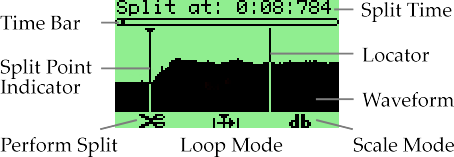
\includegraphics[width=8.0cm]{plugins/images/ss-splitedit-main-112x64x1}
      \caption{The Split Editor's Main Screen}
    \end{center}
  \end{figure}

\subsubsection{The Split Editor's Main Screen}
  \begin{description}
    \item[The waveform]
      displays the volume of the song over time. It will appear as the song
      plays and help to visually identify the point in time where the split is
      desired
      %
    \item[The split point indicator]
      is a vertical line with a small triangle at the top end. It is the most
      important control element of the split editor. It can be moved with the
      \ButtonLeft\ and \ButtonRight\ buttons. Later, when you have fine tuned
      the split point, the song will be split at this position.
      %
    \item[The split time]
      At the top of the window a time value is displayed. This is the point in
      time within the song at which the split point indicator is positioned.
      %
    \item[The locator]
      Another vertical bar represents the position locator. It moves along as
      the song plays. In contrast to the split point indicator it has no
      triangles at the ends.
      %
    \item[The time bar]
      displays the current position within the song relative to the whole song.
      The entire length of the time bar represents the song length. The length
      of the solid part of the time bar represents the position and length of
      the displayed part of the song.
      %
    \item[The scale mode]
      On the right side of the bottom line the scale mode is displayed. The
      waveform can be scaled either logarithmically or linearly. In logarithmic
      scale mode the letters ``dB'' are displayed, in linear mode ``\%''. Use
      \opt{RECORDER_PAD}{\ButtonFThree}
      \opt{ONDIO_PAD}{\ButtonMenu\ + \ButtonRight}
      to switch between these modes. Linear mode usually gives better optical
      hints with commercially recorded music. For quiet recordings,
      especially of human speech, the logarithmic scale often is preferable.
      More information in the Scale \reference{ref:Scalemode} below.
      %
    \item[The loop mode]
      In the middle of the bottom line the loop mode icon is displayed.
      There are 4 different loop modes. Pressing
      \opt{RECORDER_PAD}{\ButtonFTwo}
      \opt{ONDIO_PAD}{\ButtonMenu\ + \ButtonUp}
      changes to the next loop mode.
      %
      \begin{description}
        \item
        
\includegraphics[width=0.53cm]{plugins/images/icon-splitedit-loop-1}
          Playback loops around the split point indicator. This mode is best
          used when searching and zooming for the desired point at which to split
          the recording.
        \item
        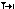
\includegraphics[width=0.53cm]{plugins/images/icon-splitedit-loop-2}
          Playback loops from the split point indicator to the end of the
          visible area. This mode is best used when fine tuning the split
          indicator position at the beginning of a recording.
        \item
        
\includegraphics[width=0.53cm]{plugins/images/icon-splitedit-loop-3}
          Playback loops from the beginning of the
          visible area to the split point. This mode is best used when fine
          tuning the split indicator position at the end of a recording.
        \item
        
\includegraphics[width=0.53cm]{plugins/images/icon-splitedit-loop-4}
          Playback does not loop, the borders of the visible
          area as well as the split point indicator are ignored. This mode is
          best used when playing the song outside of the borders of the displayed
          region.
      \end{description}
    \item[Perform the split (8)]
          The icon above the
          \opt{RECORDER_PAD}{\ButtonFOne}
          \opt{ONDIO_PAD}{\ButtonLeft}
          button indicates its function to execute the split. When split
          positioning is complete open the save dialogue with
          \opt{RECORDER_PAD}{\ButtonFOne}
          \opt{ONDIO_PAD}{\ButtonMenu\ + \ButtonLeft}.
  \end{description}

  \begin{table}
    \begin{btnmap}{Controls in the split editor}{}
      \ButtonOff & Quit plugin \\
      %
      \ButtonLeft\ / \ButtonRight &  Move the split point indicator \\
      %
      \ButtonUp\ / \ButtonDown & Zoom in / out \\
      %
      \opt{RECORDER_PAD}{\ButtonPlay}
      \opt{ONDIO_PAD}{\ButtonMenu}
      & Play from the split position \\
      %
      \opt{RECORDER_PAD}{\ButtonFOne}
      \opt{ONDIO_PAD}{\ButtonMenu\ + \ButtonLeft}
      & Enter the save dialogue \\
      %
      \opt{RECORDER_PAD}{\ButtonFTwo}
      \opt{ONDIO_PAD}{\ButtonMenu\ + \ButtonUp}
      & Toggle loop modes \\
      %
      \opt{RECORDER_PAD}{\ButtonFThree}
      \opt{ONDIO_PAD}{\ButtonMenu\ + \ButtonRight}
      & Toggle logarithmic / linear scaling \\
      \opt{RECORDER_PAD}{
      %
      \ButtonOn\ + \ButtonLeft
      & Play half speed \\
      %
      \ButtonOn\ + \ButtonRight
      & Play 150\% speed \\
      %
      \ButtonOn\ + \ButtonPlay
      & Play normal speed \\
    }
    \end{btnmap}
  \end{table}

\subsubsection{Save dialogue}
In the save dialogue it is possible to specify which of the files you
want to save and their names.  When finished, select
``Save'' and the files will be written to
disk. Note that files can not be overwritten, so filenames that
do not exist yet must be chosen. If unsure whether the
file already exists simply try to save it. If another file with this
name exists the dialogue will return and you can choose another
filename

\screenshot{plugins/images/ss-splitedit-save}{The Split Editor's
Save Dialogue}{}

\begin{table}
  \begin{btnmap}{Controls in the save dialogue}{}
    \ButtonUp\ / \ButtonDown & Select item \\
    %
    \opt{RECORDER_PAD}{\ButtonPlay}
    \opt{ONDIO_PAD}{\ButtonRight}
    & Toggle / edit item \\
    %
    \ButtonOff & Cancel \\
  \end{btnmap}
\end{table}

\subsubsection{\label{ref:Scalemode}Scale}
The values in the waveform are scaled according to the settings of the
peak meter. These can be altered in the peak meter settings,
see \reference{ref:Peakmetersetting}. If extreme minimum or
maximum values are set the waveform might be cut off.  A minimum
setting of {}-60 dB and a maximum setting of 0 dB are recommended.
These settings should be capable of producing useful waveforms for very
soft sounds in logarithmic mode (dB). When the editor is used on loud
sounds (such as commercial rock or pop music) switching to the linear
scale may prove more effective since the logarithmic scale compresses
loud noises and makes it more difficult to identify characteristic
shapes. Note that it is always possible to toggle between the two scale
modes.


